\documentclass[aspectratio=169,usenames,dvipsnames]{beamer}


\usetheme{default}  % You can choose any other theme you prefer

\title{08 - Algoritmos}
\subtitle{Dígrafos}
\author{Mateus Oliveira de Figueiredo}
\date{}

\usepackage{tikz}
\usetikzlibrary{matrix}
\usepackage{multicol}
\usepackage{algorithm}
\usepackage{algpseudocode}
\usepackage{xcolor}
\usepackage[utf8]{inputenc}
\usepackage[portuguese]{babel}
\usepackage{amsmath} % for "pmatrix" environment  
\usepackage{pgffor} 
\usepackage{listings}

\usepackage{pgfplots}
\DeclareUnicodeCharacter{2212}{−}
\usepgfplotslibrary{groupplots,dateplot}
\usetikzlibrary{patterns,shapes.arrows, positioning, arrows}
\usetikzlibrary{graphs, graphs.standard}
\pgfplotsset{compat=newest}

\lstset{
  language=Python,
  basicstyle=\ttfamily\tiny,
  keywordstyle=\color{blue},
  commentstyle=\color{green},
  stringstyle=\color{red},
  stepnumber=1,
  numbersep=10pt,
  showspaces=false,
  showstringspaces=false,
  tabsize=2,
  breaklines=true,
  breakatwhitespace=true,
}

\begin{document}

\begin{frame}
\titlepage
\end{frame}

\begin{frame}
\frametitle{Dígrafos}
\vfill
Algoritmos:
\begin{itemize}
  \item Ordem Topológica
  \item Componentes Fortemente Conexas (Kosaraju)
\end{itemize}
\vfill
\end{frame}

\begin{frame}
  \frametitle{Ordem Topológica - Gerando DAG}

  \begin{itemize}
    \item Pegue uma permutação dos nós de G para ser uma ordem topológica
    \item Adicione arestas de forma que a ordem topológica seja respeitada com determinada probabilidade
  \end{itemize}
\end{frame}

  \begin{frame}
    \frametitle{Ordem Topológica - Gerando DAG}

    \begin{itemize}
      \item Pegue uma permutação dos nós de G para ser uma ordem topológica
      \item<2> Adicione arestas de forma que a ordem topológica seja respeitada com determinada probabilidade
    \end{itemize}

    \vfill

    \begin{center}
      \begin{tikzpicture}[->,>=stealth',shorten >=1pt,auto,node distance=3cm,
                          thick,main node/.style={circle,fill=blue!20,draw,font=\sffamily\Large\bfseries}]

        \node[main node] (1) {2};
        \node[main node] (2) [right of=1] {1};
        \node[main node] (3) [right of=2] {0};
        \node[main node] (4) [right of=3] {3};

        \path<2>[every node/.style={font=\sffamily\small}, dashed]
          (1) edge[right] node [right] {} (2)
          (1) edge[bend right] node [right] {} (3)
          (1) edge[bend right] node [right] {} (4)
          (2) edge[right] node [right] {} (3)
          (2) edge[bend right] node [right] {} (4)
          (3) edge[right] node [right] {} (4);
      \end{tikzpicture}
    \end{center}

    \vfill

\end{frame}

\begin{frame}[fragile]  % The 'fragile' option is needed when code listings are included
  \frametitle{Implementação Ordenação Topológica}

  \begin{columns}
    \begin{column}{0.5\textwidth}
      \begin{lstlisting}[language=Python]
def topological_order(self, vert_start):
    marcado = [False] * self.size
    pos_ordem = []

    self.dfs(vert_start, marcado, pos_ordem)

    for i in range(self.size):
        if not marcado[i]:
            self.dfs(i, marcado, pos_ordem)

    return pos_ordem[::-1]
      \end{lstlisting}
    \end{column}
    \begin{column}{0.5\textwidth}
      \begin{lstlisting}[language=Python]
def dfs(self, vert, marcado, pos_ordem):
marcado[vert] = True

for vizinho in self.adj[vert]:
    if not marcado[vizinho]:
        self.dfs(vizinho, marcado, pos_ordem)

pos_ordem.append(vert)
      \end{lstlisting}
    \end{column}
  \end{columns}

\end{frame}

\begin{frame}{Execução em DAG completo}

  \begin{columns}[t]
  \column{0.5\textwidth}
  \begin{figure}[ht]
  \centering
  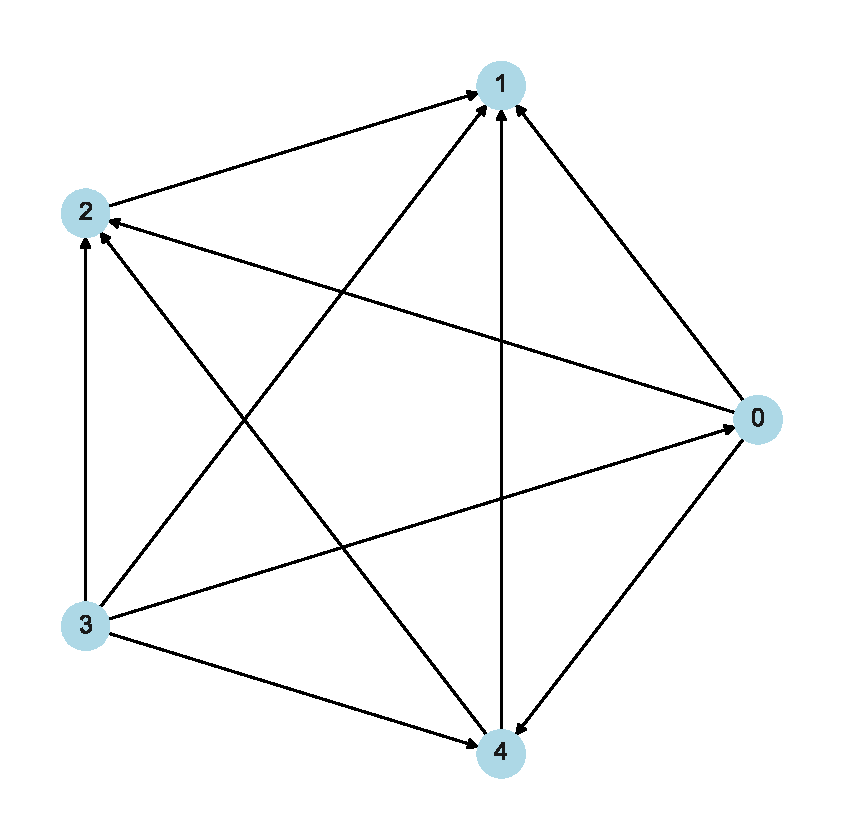
\includegraphics[width=0.9\textwidth]{figs/dag_complete_5.pdf}
  \end{figure}
  \column{0.5\textwidth}
  \vfill
  \begin{figure}[ht]
  \centering
  \includegraphics<2>[width=0.9\textwidth]{figs/dag_complete_top_5.pdf}
  \end{figure}
  \vfill
  \end{columns}
  
\end{frame}

\begin{frame}[fragile]  % The 'fragile' option is needed when code listings are included
  \frametitle{Checagem da corretude}

      \begin{lstlisting}[language=Python]

def check_topological_order(g, top_order):
    for i in range(1, g.size):
        for j in range(i):
            assert not g.are_neighbours(top_order[i], top_order[j])

      \end{lstlisting}

\end{frame}


\begin{frame}{Performance Ordenação Topológica}
  \begin{columns}
    \column{0.35\textwidth}
    
    \begin{itemize}
      \item Completo m = n(n-1)/2 
      \item m = 0(n)
    \end{itemize}

    \column{0.65\textwidth}

    \begin{figure}[ht]
    \centering
    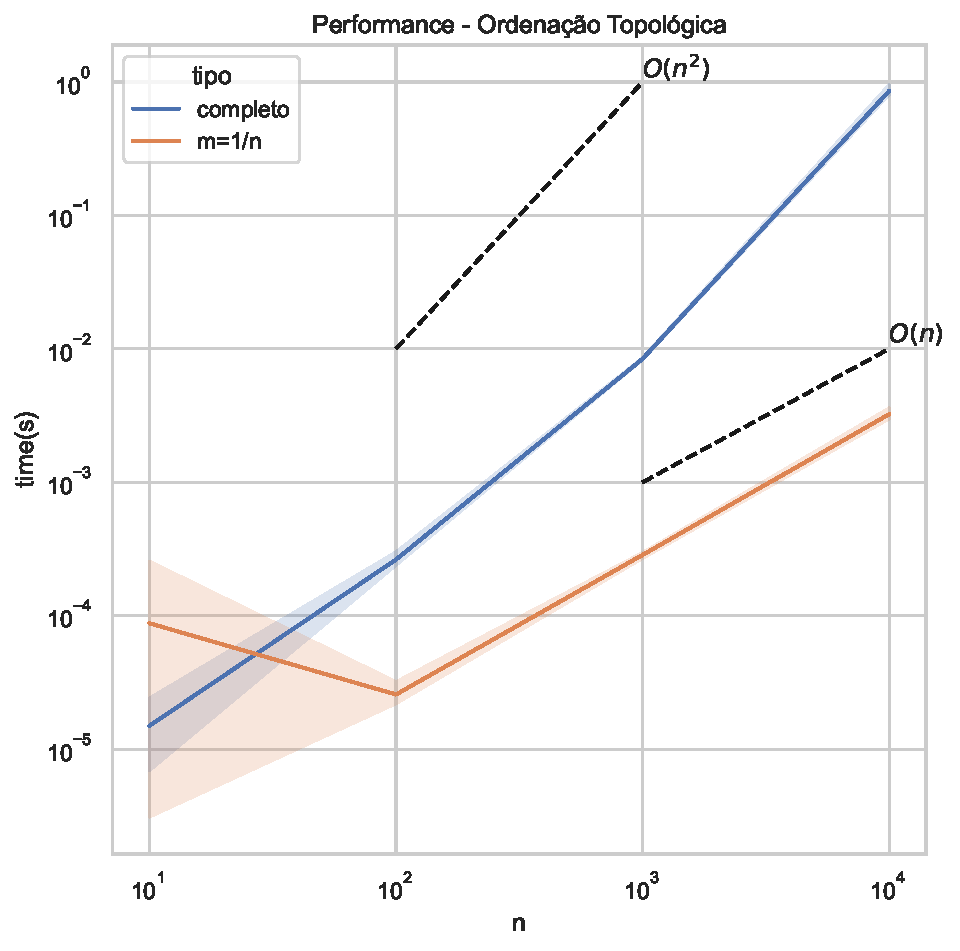
\includegraphics[width=0.9\textwidth]{figs/topological_order_time.pdf}
    \end{figure}

  \end{columns}
\end{frame}



\begin{frame}{Motivação - Algoritmo de Kosaraju}




  
\end{frame}


\begin{frame}{Algoritmo de Kosaraju}

  \begin{itemize}
    \item Realize uma DFS em $G^{R}$ e encontre uma pós-ordem reversa
    \item Faça uma DFS em $G$ na ordem da pós-ordem reversa até marcar todos os nós
    \item Cada DFS representa uma componente conexa
  \end{itemize}

\end{frame}

\begin{frame}{Exemplo Kosaraju}

  \begin{columns}
  \column{0.5\textwidth}
  \begin{figure}[ht]
  \centering
  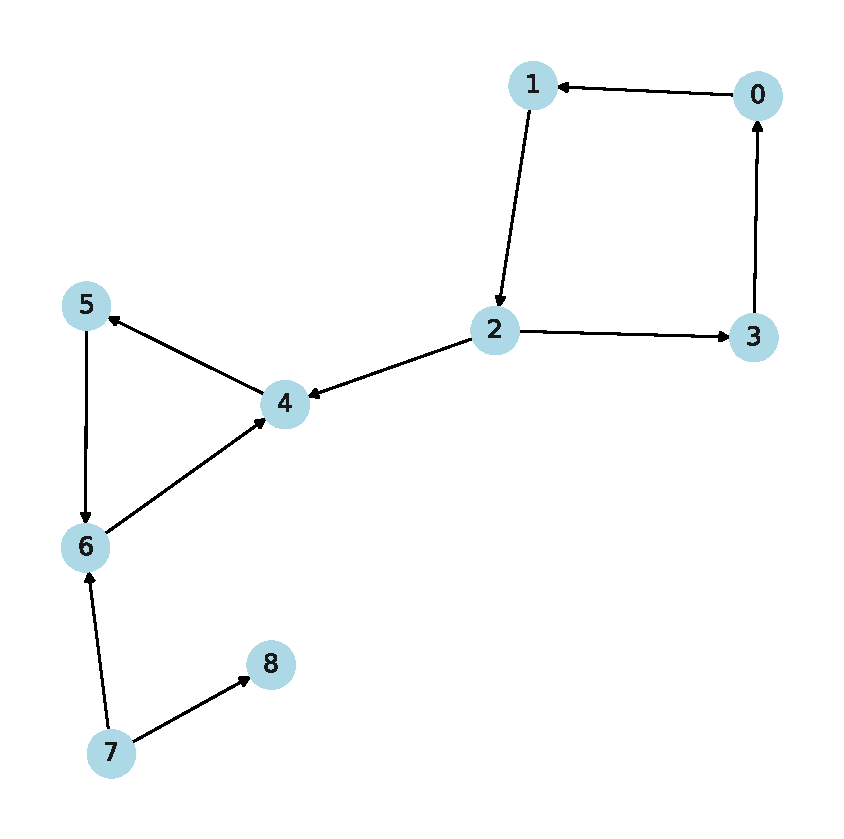
\includegraphics[width=0.9\textwidth]{figs/strongly_components_3.pdf}
  \end{figure}
  \column{0.5\textwidth}
  \begin{figure}[ht]
  \centering
  \includegraphics<2>[width=0.9\textwidth]{figs/strongly_components_4.pdf}
  \end{figure}
  \end{columns}

\end{frame}

\begin{frame}{Exemplo Kosaraju}

  \begin{columns}
  \column{0.5\textwidth}
  \begin{figure}[ht]
  \centering
  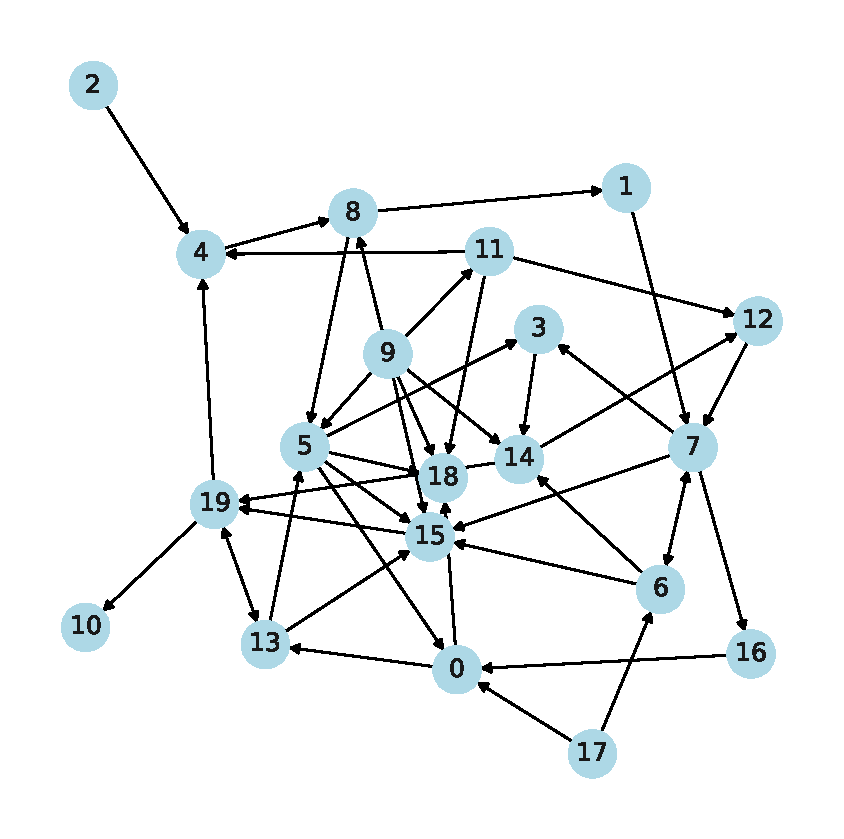
\includegraphics[width=0.9\textwidth]{figs/strong_components_0.pdf}
  \end{figure}
  \column{0.5\textwidth}
  \begin{figure}[ht]
  \centering
  \includegraphics<2>[width=0.9\textwidth]{figs/strong_components_1.pdf}
  \end{figure}
  \end{columns}

\end{frame}

\begin{frame}{Performance Kosaraju}
  \begin{columns}
    \column{0.35\textwidth}
    
    \vfill
    \begin{itemize}
      \item Completo m = n(n-1) 
      \item m = O(n)
    \end{itemize}
    \vfill

    \column{0.65\textwidth}

    \begin{figure}[ht]
    \centering
    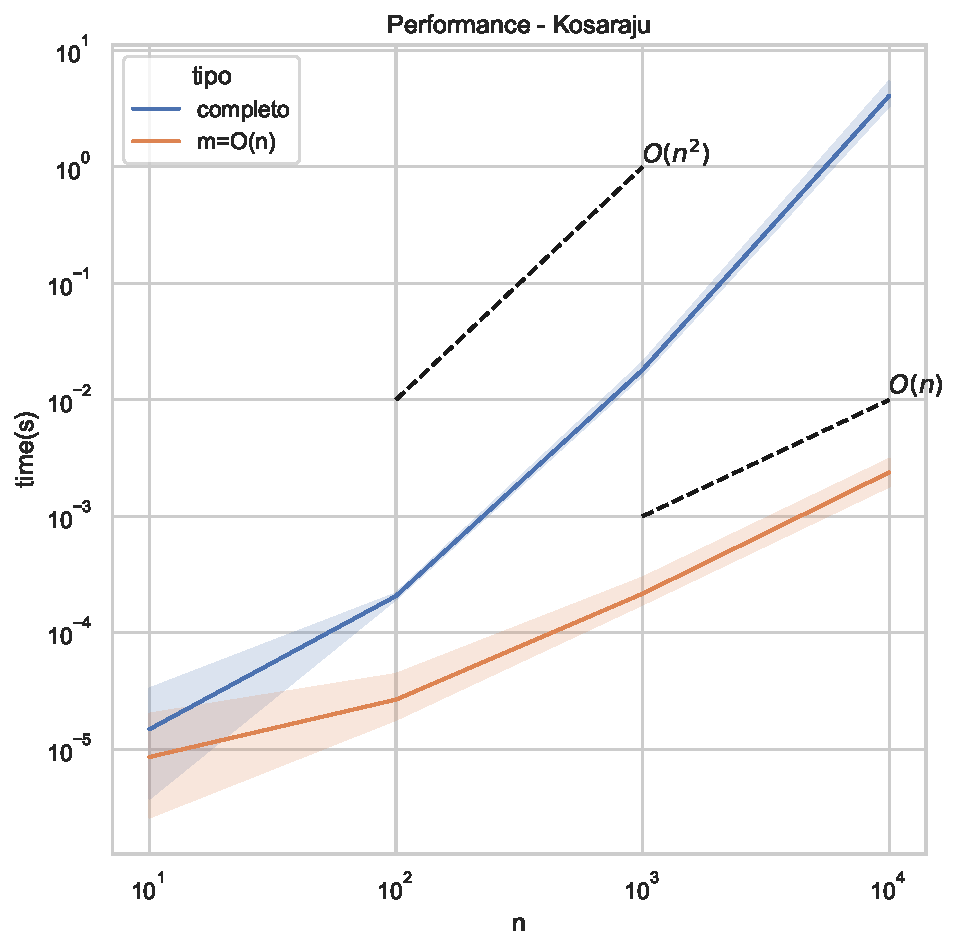
\includegraphics[width=0.9\textwidth]{figs/kosaraju_time.pdf}
    \end{figure}

  \end{columns}
\end{frame}


\end{document}
